\documentclass{sig-alternate} % Mandatory

\begin{document}

\conferenceinfo{ICSE}{'15 Florence}
\title{Drawing Representative Conclusions about Software:\\A Sampling Technique and New Spreadsheet Corpus}
%TODO title not quite right
% \numberofauthors{4}
% \author{
% Yoonki Song, Titus Barik, Brittany Johnson, and Emerson Murphy-Hill\\
% \affaddr{Department of Computer Science}\\
% \affaddr{North Carolina State University}\\
% \affaddr{Raleigh, North Carolina, USA}\\
% \{\href{mailto:ysong2@ncsu.edu}{ysong2},
%   \href{mailto:tbarik@ncsu.edu}{tbarik},
%   \href{mailto:bijohnso@ncsu.edu}{bijohnso}\}@ncsu.edu,
%   \href{mailto:emerson@csc.ncsu.edu}{emerson}@csc.ncsu.edu\\
% }

%-----------------------------------------------------------------------------%
\maketitle

\begin{abstract}
Spreadsheets users are the largest group of software developers on
the planet, and much of what researchers know about this group derives
from the EUSES corpus, a corpus that includes about 5,000 spreadsheets
mined from the web a decade ago.
While the EUSES corpus has yielded many interesting research results,
the corpus is aging and small, relative to the number of spreadsheets
used today.
Moreover, the EUSES corpus was obtained entirely from spreadsheets posted
to the public web.
In this paper, we introduce several new spreadsheet corpora: one corpus contains
about 1.5 million open-source spreadsheets mined from the public web, 
and three others mined from formerly closed-source email attachments from the Stratfor intelligence
company, the Enron energy firm, and the Syrian government.
%TODO
We also use these corpora to introduce a new sampling techinque that allows researchers to 
create their own open-source software corpus that is representative of 
a a closed-source corpus.
%TODO what follows is technically an eval -- does our technique produce more representative
%	corpus with respect to three studies?
We evaluate the utility of our technique by 
replicating part of a recent spreadsheet study and showing
how results from subsampled open-source are equivalent to 
results obtained from the original closed-source corpus.
%TODO add some interesting results
\end{abstract}

\section{Introduction}

Spreadsheets are an important type of software development.
-how many people use them,
-examples of errors and their impact (e.g, Reinhard and Rogoff)

There's existing rich-reasearch on spreadsheets.
Examples.

\subsection{State of the art}
Currently, the most used corpus for spreadsheet analysis is the EUSES corpus. This corpus contains spreadsheets obtained mainly by searching in search engines, so it contains spreadsheets that are publicly available. However, industrial case studies performed by us and other researchers have raised questions about the representativeness of this corpus, as spreadsheets we  encounter in industry tend to be bigger and be more complex. Hence, we believe there is a need for a corpus providing a more realistic test set for spreadsheet researchers.

Where corpus comes from, how it was derived, how many spreadsheets.


Examples, probably from threats sections.
Impact: if not representative, conclusions do not generalize.
Example from prior paper.

In this paper, we present a technique that enables researchers
to draw more generalizable conclusions in their studies.
In a nutshell, the technique involves\ldots

Although this paper focuses on spreadsheets, in reality 
spreadsheets are a microcosm of broader software development,
and consequently the techniques presented here can be used for other 
types of software as well.

The contributions of this paper are:

\begin{itemize}
  \item A technique for creating representative samples of open-source
  		software;
  \item An open-source corpus of spreadsheets more than two orders of magnitude larger
 		than the existing state of the art, along with a never-before analyzed
 		pseudo-closed-source corpus;
  \item A set of distributions of real closed-source spreadsheets that can be
  		used as parameters to our technique; and
  \item An evaluation that suggests our technique can produce more representative
  		results than using the existing state of the art corpus.
\end{itemize}

\section{Prior Work}

Maybe a bit more depth in spreadsheet research, showing how serious it is.

A good bit from Mei Nagappan's representativeness paper~\cite{nag13}.

\section{Our Technique}

Based on that sampling thing represented by the stats professor.

Section closing: talk about you need a good corpus to sample from.

\section{Our Open-Source Corpus}

We took this opportunity to update the old corpus, using roughly similar
methodology.

\subsection{Mining Methodology}

How we mined the web.

\subsection{Corpus Characterization}

Number of spreadsheets, a few stats about them.

Distribution comparison to EUSES here?

\begin{figure}
\centering
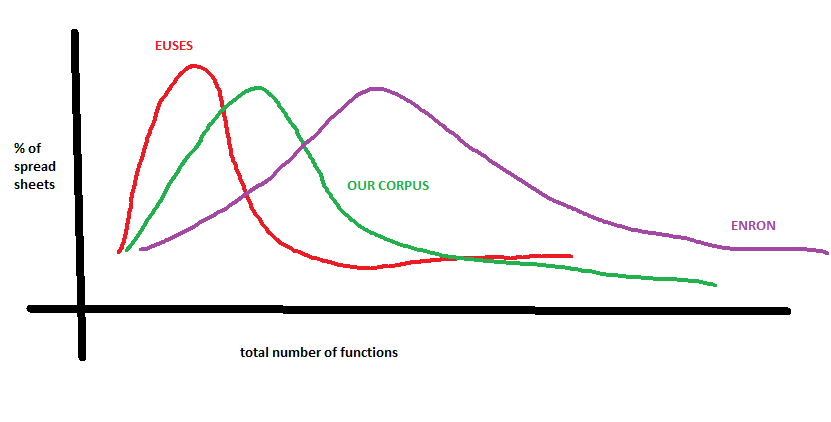
\includegraphics[width=\columnwidth]{functions.png}
\caption{Distribution of number of fuctions per spreadsheet, for 3 spreadsheet corpuses.}
\label{fig:effectiveness}
\end{figure}

\section{The Enron Data Set}

While the sample of the Google spreadsheets provides us with a better set than the current EUSES corpus, it still misses the context of real-life industry spreadsheets. Therefore we present a second data set in the paper, derived from the Enron E-mail Archive. This is an large database of over 600,000 emails containing emails from by 158 Enron employees, which was purchased and released by researchers at the University of Massachusetts Amherst. 

\subsection{Data}
First, we requested the most recent version of the dataset, via this form. We got access to v1.3, last updated 29 July, 2013. This version contains 130 folders (one per employee, each containing one or more pst file) with 190 pst files, and is 53 gigs in size.

\subsection{Getting the spreadsheets}
Using the systool's outlook attachment extractor TODO: link, we obtained the spreadsheets from the pst. With the extractor, obtaining all spreadsheets took about 6 hours, on an i7 machine with 16 gig memory. In total, the email set contains 265,586 files (32.3 gigs), of which over 50.000 are Excel files. Among those files are 11.985 unique spreadsheets.

\subsubsection{Analysis}
For all the spreadsheets, we ran the Spreadsheet Scantool, developed at Delft University of Technology. This tool runs on the previously developed Breviz core, made for spreadsheet visualization and smell detection. TODO: References. 11.136 spreadsheets could be analyzed, the others were corrupt, password protected, or otherwise unreadable.

\subsection{The spreadsheets}
\subsubsection{Worksheets}
In total, the 11.136 spreadsheets contain 49,872 worksheets. This is a aveage of 4.4 worksheets per spreadsheet. Most spreadsheets have 3 worksheets, most likely because this is the default number of worksheets in 

\section{Conclusion}

\section{Distributions from Real Closed-Source Code}

Describe dataset.
Talk about distribution. (plot distribution on same axis, maybe three different metrics).

\section{Evaluation}

RQ1: Are distributions statistically significantly different for the spreadsheet sets discussed here?
RQ2: Do the conclusions from existing studies change depending on what corpus they use? (Compare uses to others)
RQ3: Do conclusions drawn using our sampling technique better approximate conclusions from original sample?

\subsection{RQ1}

\subsection{RQ2}

We next replicate three prior studies about spreadsheets in our new corpora,
with an aim towards understanding how results differ when different corpora are
used for evaluation purposes.

\subsection{CheckCell}

Our first replication is an evaluation of Barowy, Gochev, and Berger's
CheckCell tool~\cite{Barowy14}, a tool that was built to identify spreadsheet
cells that have an inordanately high impact on calculations.
The intuition is that such cells may contain data input errors.

As part of their evaluation, CheckCell's authors wanted to know whether checkcell runs efficiently
To evaluate efficiency, the authors randomly selected 64 spreadsheets that contained at least one
formula from the EUSES corpus, then ran their analysis on a commodity laptop.
They conclude, ``For most of the spreadsheets, CheckCell completes its analysis in under 50 seconds;
for all but two, it completes in under five minutes.''
The results for all spreadsheets are shown as blue bars on Figure~\ref{fig:effectiveness}.

\begin{figure}
\centering
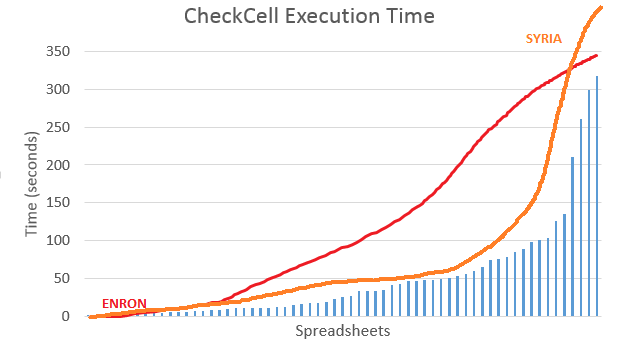
\includegraphics[width=\columnwidth]{checkcell.png}
\caption{CheckCell efficiency data.}
\label{fig:effectiveness}
\end{figure}

We first used our VCL infrastructure to run CheckCell on all EUSES spreadsheets; we assume
that Borowy and colleagues did not do this originally for efficiency reasons.
We then ran the results on each of our other data sets.
The results are overlaid on Figure~\ref{fig:effectiveness}.
We then performed an unpaired t-test to determine whether there were significant differences
in the distributions.
%TODO probably want ot make sure distributions are normal first

The results suggest that:
- Outcome 1: No significant differences. Does this diminish the need for our technique?
	Perhaps we can say that our approach confirms that Bowory's sampling was reasonable,
	and that euses is a good 
- Outcome 2: No differences between open source sets, but some between open and closed. 
	Tells us that the closed ones are systematically different.
- Outcome 3: Differnece between open source sets. The most interesting! Says something about
	sampling methods.

\subsection{RQ3}

\section{Limtations}

Limitations of both the technique, and the study.

\section{Conclusions}

\end{document}
